\begin{figure}[H]
\centering
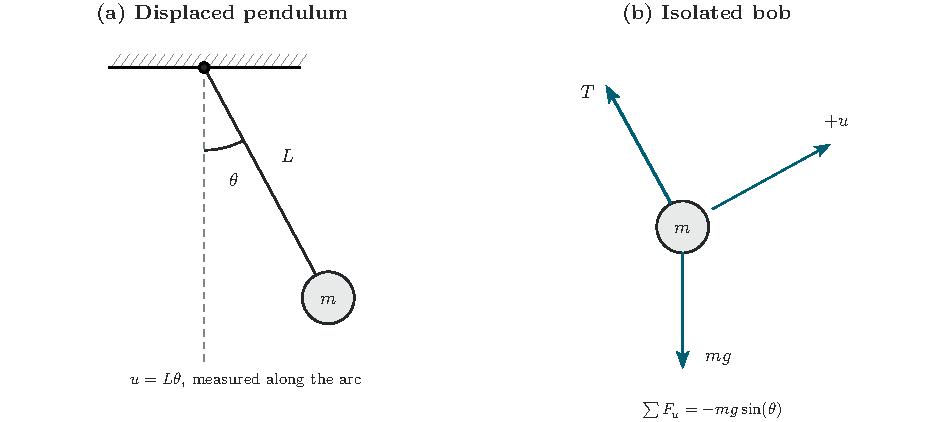
\includegraphics[width=0.95\linewidth,height=\textheight,keepaspectratio,alt={Free-body diagram for Problem A.1.}]{figures/generated/solutions/pendulum_fbd.pdf}
\caption{Free-body diagram for Problem A.1.}
\end{figure}

The derivation below follows the class notes on pages 5--10 and the general free-vibration derivation on pages 18--19. The notation is adapted so that \(\theta\) denotes angular displacement and \(u\) denotes tangential particle displacement.

Assume a point mass, a massless inextensible rod or taut string of length \(L\), a fixed frictionless pivot, uniform gravity, planar motion, and negligible air resistance. Measure \(\theta\) from the downward vertical. Let \(u=L\theta\) be arc displacement. This relation is exact for arc displacement; horizontal displacement is \(L\sin\theta\approx u\) only for small angles.

The free-body diagram has weight \(mg\) downward and tension \(T\) toward the pivot. Tension has no tangential component. Gravity contributes the restoring tangential force \(-mg\sin\theta\). Newton's law of motion therefore gives

\[mL\ddot\theta=-mg\sin\theta.\]

For \(|\theta|\ll1\) in radians, \(\sin\theta\approx\theta\), so the linear equation of motion and its mass-normalized governing equation are

\[\boxed{mL\ddot\theta+mg\theta=0}\qquad\text{(A.1.4)}\]

\[\boxed{\ddot\theta+\frac{g}{L}\theta=0}\qquad\text{(A.1.5)}\]

Substitute \(\theta=e^{st}\) and use \(\ddot\theta=s^2e^{st}\). Since the exponential is nonzero, its coefficient must vanish. The characteristic equation is

\[\boxed{s^2+\frac{g}{L}=0}\qquad\text{(A.1.7)}\]

The roots are purely imaginary, so the correct choice for item 8 is

\[\boxed{\text{Purely imaginary roots}}\qquad\text{(A.1.8.a)}\]

Define the natural angular frequency as

\[\boxed{\omega_n=\sqrt{\frac{g}{L}}}\qquad\text{(A.1.9)}\]

The roots are then

\[\boxed{s_1=i\omega_n,\qquad s_2=-i\omega_n}\qquad\text{(A.1.10)}\]

The angular solution can be written in either equivalent form

\[\boxed{\theta(t)=D_1e^{i\omega_nt}+D_2e^{-i\omega_nt}}\qquad\text{(A.1.11)}\]

\[\boxed{\theta(t)=A_\theta\cos(\omega_nt)+B_\theta\sin(\omega_nt)}\qquad\text{(A.1.12)}\]

The frequency in hertz and oscillation period are

\[\boxed{f_n=\frac{\omega_n}{2\pi}=\frac{1}{2\pi}\sqrt{\frac{g}{L}}}\qquad\text{(A.1.13)}\]

\[\boxed{\tau=\frac{1}{f_n}=\frac{2\pi}{\omega_n}=2\pi\sqrt{\frac{L}{g}}}\qquad\text{(A.1.14)}\]

Multiplication by \(L\) gives the particle-motion solution

\[\boxed{u(t)=C_1e^{i\omega_nt}+C_2e^{-i\omega_nt}}\qquad\text{(A.1.15.a)}\]

\[\boxed{u(t)=A\cos(\omega_nt)+B\sin(\omega_nt)
=C\sin(\omega_nt+\varphi)}\qquad\text{(A.1.15.b)}\]

The last form is the amplitude--phase form used in the class notes. For a real-valued response, \(A\) and \(B\) are real, with

\[C=\sqrt{A^2+B^2},\qquad \varphi=\operatorname{atan2}(A,B).\]

To solve the initial value problem, evaluate both displacement and its derivative at zero. This gives \(u(0)=A=u_0\) and \(\dot u(0)=\omega_nB=v_0\), where \(v_0=\dot u_0\).

For an initial-displacement release, \(u(0)=u_0\) and \(\dot u(0)=0\), so

\[\boxed{u(t)=u_0\cos(\omega_nt)}\qquad\text{(A.1.16.i)}\]

For an initial-velocity release, \(u(0)=0\) and \(\dot u(0)=v_0\), so

\[\boxed{u(t)=\frac{v_0}{\omega_n}\sin(\omega_nt)}\qquad\text{(A.1.16.ii)}\]

Applying both initial conditions gives

\[\boxed{u(t)=u_0\cos(\omega_nt)+\frac{v_0}{\omega_n}\sin(\omega_nt)}\qquad\text{(A.1.16.iii)}\]

In exponential form the same constants are

\[C_1=\frac12\left(u_0-\frac{iv_0}{\omega_n}\right),\qquad
C_2=\frac12\left(u_0+\frac{iv_0}{\omega_n}\right).\]

Mass cancels because it multiplies both inertia and weight. A heavier ideal pendulum has the same small-angle frequency at the same length. This does not mean mass cancels from an impact calculation.
